\documentclass[journal]{IEEEtran}
%=====================================================================
\usepackage{amsmath,epsfig}
\usepackage{caption}
\usepackage{subcaption}
%\usepackage[margin=10pt]{subfig}
\usepackage{color}
%\usepackage{placeins}
\usepackage{float}
\usepackage{tabularx,colortbl}
\usepackage{amssymb}
\usepackage{amsmath,graphicx}
\usepackage{algorithm}
\usepackage{amsfonts}
\usepackage[noend]{algpseudocode}
%\usepackage{multirow} %
\usepackage{bm}
\usepackage{eqnarray}
\usepackage{algpseudocode}
%\usepackage{threeparttable}
\usepackage{hyperref}
\usepackage{epsfig}
\usepackage{verbatim}
\usepackage{times}
%\setcounter{tocdepth}{3}
\usepackage{amsthm}
\usepackage{empheq}
\usepackage{euscript}
\usepackage{fixltx2e}
%\usepackage{isomath}
%\usepackage[]{algorithmicx}
\usepackage{amsthm}

\usepackage{booktabs}
%https://tex.stackexchange.com/questions/43993/ieee-latex-style-grouping-references
\usepackage[noadjust]{cite}
%\usepackage{balance}
%https://tex.stackexchange.com/questions/49918/how-to-level-columns-in-bibliography
\usepackage{flushend}

\usepackage[dvipsnames]{xcolor}

\newtheorem{theorem}{Theorem}[section]
\newtheorem{lemma}[theorem]{Lemma}
\newtheorem{proposition}[theorem]{Proposition}
\newtheorem{corollary}[theorem]{Corollary}
% Definition Styles
\theoremstyle{definition}
\newtheorem{definition}{Definition}[section]
\newtheorem{example}{Example}[section]
\theoremstyle{remark}
\newtheorem{remark}{Remark}
\DeclareMathOperator*{\argmin}{arg\,min}
\newcommand{\change}[1]{\textcolor{black}{#1}}


%=======================================================================================
\ifCLASSINFOpdf
\else
   \usepackage[dvips]{graphicx}
\fi
\usepackage{url}

\hyphenation{op-tical net-works semi-conduc-tor}

\usepackage{graphicx}
\usepackage{amsmath,amssymb}

\begin{document}

\title{Graph Learning from Binomial Signals'}
\author{Skip Moses, Jing Guo
\thanks{This work was supported by the  Research, Scholarship, and Creative Activity (RSCA) Award from CSU, Chico. }
\thanks{Skip Moses is currently a graduate student in the College of Science and Mathematics, California Polytechnic University, San Luis Obispo, CA 93407 USA (e-mail: skipmoses@gmail.com).}
\thanks{The corresponding author Jing Guo is with the Department of Mathematics and Statistics, California State University, Chico, CA 95929 USA (e-mail: jguo2@csuchico.edu).}}

\markboth{IEEE SIGNAL PROCESSING LETTERS, Vol. X, 2023}
{Shell \MakeLowercase{\textit{et al.}}: Bare Demo of IEEEtran.cls for IEEE Journals}
\maketitle

\begin{abstract}
Data often has an underlying structure of Geometry that can be modeled as a signal on the vertices of a weighted, undirected graph. There are several analogies between traditional signal processing and algebraic graph theory that translates many of the tools of discrete signal processing such as spectral analysis of multichannel signals, system transfer function, and digital filter design to name a few. Historically, GSP has focused on modeling smooth signals on a graph, but the increase in the availability of abstract data sets has motivated algorithms for learning a valid graph given a set of signals. In this work, we attempt to design a novel methodology for learning a valid graph topology given a set of binary signals on the graph. This is accomplished by extending the ideas of  Logistic Regression and Maximum Likelihood with constraints that enforce a valid graph topology on the regression coefficient matrix. 
\end{abstract}

\begin{IEEEkeywords}
graph learning, graph signal processing, binary signals, logistic regression, Laplacian matrix
\end{IEEEkeywords}

\section{Introduction}

\IEEEPARstart{D}{ata} often has an underlying structure or geometry that can be modeled as a signal on the vertices of a weighted, undirected graph. Traditionally, the emphasis was on using an underlying graph, or network, to understand the properties of signals over the vertices. Recently, there has been a surge in the converse problem; of learning a graph structure from a set of signals satisfying some constraints \cite{xia2021graph} \cite{stankovic2019vertex} \cite{ortega2018graph}. A subset of graph learning that focuses on graph signal processing-based methods deals with sampling, graph recovery, and learning topological structure \cite{xia2021graph}. 

The methods for learning topological structure fall into the categories of regression-like models \cite{dong2016learning}, \cite{tugnait2021sparse}, \cite{pu2021learning}, and \cite{saboksayr2021accelerated}, and machine learning techniques \cite{pu2021kernel}, \cite{kalofolias2016learn}, and  \cite{venkitaraman2019predicting}. In all of these models, signals are assumed to follow multivariate Gaussian distributions, but there has been little exploration into learning a network from binomial signals. 

In this work, we suppose the odds of a node having a signal value of $1$ or $0$ depend on the signal value of its neighboring nodes in order to estimate the underlying graph topology. Our methodology generalizes the framework of traditional logistic regression in order to learn an adjacency matrix from a set of binary signals.

\section{Related Work}

Dong et al. propose a modified factor analysis model in \cite{dong2016learning} for learning a valid graph laplacian. The model proposed is given by 

$$
	x = \chi h + \mu_x + \epsilon
$$

where $h \sim \mathcal{N}(0, \Lambda^{\dagger})$ is the latent variable,$\Lambda$ is the eigenvalue matrix of $L$, and  $\mu_x \in \mathbb{R}^N$ mean of $x$. The noise term $\epsilon$ is assumed to follow a multivariate Gaussian distribution with mean zero and covariance $\sigma_\epsilon^2I_N$. The key difference from traditional factor analysis is the choice of $\chi$ as a valid eigenvector matrix for a graph laplacian. Finding a maximum a posterior estimate of $h$ reduces to solving the optimization problem

\begin{equation}
	\label{eq:dongmodel}
	\begin{aligned}
		\min_{L \in \mathbb{R}^{N\times N}, \phantom{..} Y \in \mathbb{R}^{N\times P}} ||X&-Y||_F^2 + \alpha \text{tr}(Y^TLY) + \beta||L||_F^2 \\
		\textrm{s.t.}& \quad \text{tr}(L) = N, \\
		&\quad L_{i,j} = L_{j,i} \leq 0, \phantom{..} i \neq j, \\
		&\quad L\cdot \textbf{1} = \textbf{0} \\
	\end{aligned}
\end{equation}

Because (\ref{eq:dongmodel}) is not jointly convex, Dong et al. employ an alternating minimization scheme to solve the problem. Initially, set $Y = X$ and we find a suitable $L$ by solving 
\begin{equation}
	\label{eq:dongprob1}
	\begin{aligned}
		\min_L       & \phantom{..} \alpha \text{tr}(Y^TLY) + \beta ||L||_F^2, \\
		\textrm{s.t.}& \quad \text{tr}(L) = N,\\
					 & \quad L_{i,j} = L_{j,i} \leq 0, \phantom{..} i \neq j, \\
					 & \quad L\cdot \textbf{1} = \textbf{0}
	\end{aligned}
\end{equation}

Next, using $L$ from (\ref{eq:dongprob1}), we solve 
\begin{equation}
	\label{eq:dongprob2}
	\begin{aligned}
		\min_Y \phantom{..} ||X-Y||_F^2 + \alpha \text{tr}(Y^TLY)
	\end{aligned}
\end{equation}

Both (\ref{eq:dongprob1}) and (\ref{eq:dongprob2}) can be cast as convex optimization problems. Specifically, \ref{eq:dongprob1} can be solved with the alternating direction method of multipliers (ADMM). The model is applied to both synthetic and real-world data, and compared to a technique used in machine learning that is similar to sparse inverse covariance estimation of Gaussian Markov Random Field models. Four evaluation criteria were used to evaluate the performance of the framework: $\textit{Precision, Recall, F-measure,}$ and $\textit{Normalized Mutual Information (NMI)}$. Kalofolias cites two weaknesses to this model: The use of the Frobenius norm on the Laplacian has reduced interpretability, and it requires four constraints on the solution space \cite{kalofolias2016learn}. These extra constraints make computational scalability difficult.

In \cite{kalofolias2016learn}, Kalofolias provides complementary ideas to improve on the work of Dong et al. In particular, Kalofolias considers the more natural problem of learning the weighted adjacency matrix $A$, and show an extra smoothness condition leads to the learned graph being sparse. Define, $Z$ to be the matrix of pairwise distances of the signal, namely, $Z_{i,j} = ||x_i - x_j||^2$. Under this definition, we can recast our smoothness term as 
\begin{equation}
	\label{eq:kalotransform}
	\text{tr}(X^TLX) = \frac{1}{2} \text{tr}(AZ) = \frac{1}{2}  ||A\circ Z||_{1,1};
\end{equation}
where $\circ$ is the hadamard product and $||A||_{1,1}$ is the element wise 1-norm. We can now recast \ref{eq:GLP} as 
\begin{equation}
	\label{eq:GLP}
	\begin{aligned}
		\min_A       & \phantom{..} ||A\circ Z||_{1,1} + f(A), \\
		\textrm{s.t.}& \quad ||A||_{1,1} = N,\\
		& \quad A_{i,j} = A_{j,i} \geq 0, \phantom{..} i \neq j, \\
		& \quad \text{diag}(A) = \textbf{0}
	\end{aligned}
\end{equation}

The model proposed by Kalofolias is given by specifying $f(A) = -\alpha \textbf{1}^T\log(A\textbf{1}) + \beta||A||_F^2$. An appealing feature of this model is the fact that for any $\lambda >0$ and solution $F(Z,\alpha, \beta)$ the following equalities hold
\begin{equation}
	\label{eq:KalofoliasEquality}
	F(Z, \alpha, \beta) = \lambda F(Z, \frac{\alpha}{\lambda}, \beta \lambda) = \alpha F(Z, 1, \alpha \beta).
\end{equation}
This means we can fix a scale $||A|| = s$ for an arbitrary norm and solve for $\beta$ in \ref{eq:kalotransform} with $\alpha = 1$, and then re-normalize our solution. Furthermore, the log barrier term only acts on the degrees. This provides an advantage over the model \ref{eq:dongmodel}, because it promotes connectivity in the learned graph. Kalofolias goes onto show \ref{eq:kalotransform} can be solved efficiently for many choices of $f(A)$ via primal dual algorithms. 

In \cite{venkitaraman2019predicting} machine learning concepts are employed to learn a graph from training data. Let $\{x_n\}_1^N$ be a set of $N$ input observations with each $x_n$ paired with a target $t_n \in \mathbb{R}^M$. The authors model a set of smooth signals $y_n$ and $t_n$ via the following: 
\begin{equation}
	\label{eq:LinearModel}
	y_n = \textbf{W}^T\phi(x_n),
\end{equation}
where $\phi(x_n)$ is some known function and $\textbf{W}$ denotes the regression coefficient matrix. Venkitarman et al. assume only the target $y_n$ is smooth over the graph. The input $x_n$ does not have to be a signal over the graph and can even be agnostic to a graph. The cost function for the model, when the underlying graph is known, is given by 
\begin{equation}
	\label{eq:cost}
	C(\textbf{W}) = \sum_{n=1}^N\left( ||t_n - y_n||_2^2 + \beta y_n^TLy_n \right) + \alpha \text{tr}(\textbf{W}^T\textbf{W}).
\end{equation}
Next, it is shown KRG induces a smoothing effect on the target by a shrinkage in the direction of eigenvectors of $L$ that have eigenvalues less than $\alpha$. To learn an unknown graph, a term is added to the cost function $C(\textbf{W}, L) = C(\textbf{W}) + \nu \text{tr}(L^TL)$.  Venkitarman et al. uses the model to predict temperature using air-pressure observations collected in Sweden, next-day temperature from the current day in Sweden, and fMRI voxel intensities of the cerebellum region. The latter two experiments are compared to the method of kernel-ridge regression (KRR) by using a normalized-mean-square error to measure the performance of the prediction. It is concluded that the method is well suited for training with noise data sets that may be small \cite{venkitaraman2019predicting}.

\section{Preliminaries}

A weighted, undirected graph is a triple $G = (V, E, \omega)$ of two sets $V = \{1, \ldots, |V| = N \}$ and $E \subset V \times V$ and a weighting function $\omega(i,j) = \omega_{i,j}$ that assigns a non-negative real number to each edge. We can represent a graph by its adjacency matrix $A$ where $A_{i,j} = \omega_{i,j}$ if $(i,j) \in E$ and $0$ otherwise. A signal on a graph $G$ is a function $f: V \rightarrow \mathbb{R}$ that can be represented as vector $x \in \mathbb{R}^N$. The Laplacian of a graph is the matrix $L = D - A$ where $D$ is the degree matrix. The Laplacian acts as a difference operator on signals via it's quadratic form
\begin{equation}
	\label{eq:quadraticform}
	x^TLx = \sum_{(i,j)\in E}A_{i,j}(x_j - x_i)^2.
\end{equation} 
The Laplacian is positive and semi-definite, so it has a complete set of orthonormal eigenvectors and real nonnegative eigenvalues. Thus, we can diagonalize $L = \chi^T\Lambda \chi$ where $\Lambda$ is the diagonal matrix of eigenvalues and $\chi$ is the associated matrix of eigenvectors. 

Note that \ref{eq:quadraticform} is minimized when adjacent vertices have identical signal values. This makes \ref{eq:quadraticform} well suited for measuring the smoothness of a signal on a graph. We can cast the problem of learning a graph by the optimization problem found in \cite{kalofolias2016learn}
\begin{equation}
	\begin{aligned}
		\min_L       & \phantom{..} \text{tr}(Y^TLY) + f(L), \\
		\textrm{s.t.}& \quad \text{tr}(L) = N,\\
		& \quad L_{i,j} = L_{j,i} \leq 0, \phantom{..} i \neq j, \\
		& \quad L\cdot \textbf{1} = \textbf{0}
	\end{aligned}
\end{equation}


\section{Methods}

\subsection{Signals on the graph and model specification}

We consider a weighted undirected graph $G = (V, E)$, with the vertices set $V = {1, 2, \dots, N}$, and edge set $E$.  Let $\mathbf{A}$ denote the weighted adjacency matrix of $G$. In the case of a weighted undirected graph, $\mathbf{A}$ is a square and symmetric matrix. 

Let $\mathbf{Y}_{i,j}$ denote the signal on the node $i$ of graph $G$ at round $j$, where $j = 1, \dots, M$, and $i = 1, \dots, N$. We assume that $\mathbf{Y}_{i,j}$ is a binary signal that can be 1 or 0. 
Suppose the signals at stratum $j$ denoted by $\mathbf{Y}[, j]$ for all $N$ nodes are independent of the signals at stratum $k$ denoted by $\mathbf{Y}[,k ]$, for $j \neq k$. Let $p_{i,j}$ denote the probability of $\mathbf{Y}_{i,j} = 1$. Our model assumes

\begin{equation}
\label{eq: binaryglm}
\text{logit}(p_{i,j}) = (\mathbf{A} h )_i,
\end{equation}

where $\mathbf{A}$ is the adjacency matrix from the graph $G$, $h$ is a vector of latent factors that governs $p_{i, j}$ through $\mathbf{A}$ and assumed to be a standard normal random vector. 

\subsubsection{Maximum likelihood for one stratum}

Consider the probability mass function for a given $\mathbf{A}$ and signal $y = \mathbf{Y}[,k]$
\begin{align}
P_{\mathbf{A}h}(y_i) &= p^{y_i}(1-p)^{1-y_i} \\
            &= \left(\frac{e^{\mathbf{A}[i,]h}}{1 + e^{\mathbf{A}[i,]h}}\right)^{y_i}\left(1- \frac{e^{\mathbf{A}[i,]h}}{1 + e^{\mathbf{A}[i,]h}}\right)^{1-y_i} \\
            &= \left(\frac{e^{\mathbf{A}[i,]h}}{1 + e^{\mathbf{A}[i,]h}}\right)^{y_i}\left(\frac{1}{1 + e^{\mathbf{A}[i,]h}}\right)^{1-y_i}   \\
            &= \frac{e^{y_i\mathbf{A}[i,]h}}{1 + e^{\mathbf{A}[i,]h}}
\end{align}

Therefore, our likelihood function will be given by 

\begin{align}
\mathcal{L}(h) = \prod_{i=1}^N\left(\frac{e^{y_i\mathbf{A}[i,]h}}{1 + e^{\mathbf{A}[i,]h}}\right)
\end{align}

In order to maximize we consider the natural logarithm of our likelihood

\begin{align}
\log(\mathcal{L}(h)) = \sum_{i=1}^N\left(y_i(\mathbf{A}[i,]h) - \log(1 + e^{\mathbf{A}[i,]h})\right)
\end{align}

\subsubsection{Optimization Program}

Taking inspiration from the above derivation we will solve for estimated $\mathbf{A}$ by maximizing the following

\begin{equation}
\label{eq:optimization}
\begin{aligned}
\max_{\mathbf{A},h} \phantom{..}& \sum_{j = 1}^M\sum_{i=1}^N\left(y_{i,j}(\mathbf{A}[i,]h) - \log(1 + e^{\mathbf{A}[i,]h})\right) - \alpha \vert L \vert _ F \\
\textrm{s.t.}  & \quad \mathbf{A}_{i,j} = 0 \text{ if } i =j \\
               & \quad \mathbf{A}_{i,j} \geq 0 \text{ if } i \neq j\\
               & \quad h \sim \mathcal{U}(-1,1) 
\end{aligned}
\end{equation}
where $\alpha$ is a tuning parameter for controlling the sparsity and $a$ and $b$ are tuning parameters for restricting the spread of the values of $h$. 

\subsubsection{Algorithm}

We present our optimization algorithm below. In each iteration of steps 5) and 6) of Algorithm 1, the optimization program gives a Disciplined Concave Program that can be solved efficiently in Python with the CVXPY library.

\begin{align*}
&\textbf{Algorithm 1: Binary Signal Graph Learning} \\
&1) \textbf{ Input: } \text{ Input binary signals on a graph } \mathbf{Y}.\\
&2) \textbf{ Output: } \text{ Output an estimated } \mathbf{A}.\\
&3) \textbf{ Initialization: } h_{i,0} \sim \mathcal{U}(-1,1) \text{ for } i = 1,\ldots, N \\
&4) \textbf{ for } t = 1, \ldots, iter:\\
&5) \textbf{ Update } \mathbf{A} \textbf{ given } h:\\
&6) \,\,\,\, \textit{ Fix }  h \textit{ in Optimization Program and solve } \mathbf{A} \\
&7) \textbf{        Update } h \textbf{ given } \mathbf{A}:\\
&8) \,\,\,\, \textit{ Fix } \mathbf{A} \text{ in Optimization Program and solve h} \\
&9) \textbf{ end for }
\end{align*}

\section{Results}

\subsection{Synthetic Data Generation}

\begin{figure}
  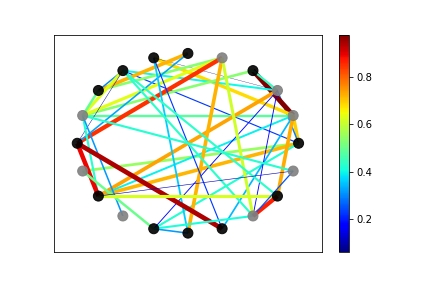
\includegraphics[width=\linewidth]{pictures/gt_graph.png}
  \caption{Ground truth graph used to generate synthetic data.}
  \label{fig:gt}
\end{figure}

Let $\mathbf{A}$ be the adjacency matrix of the graph in Figure \ref(fig:GTG), and $h \in \mathbb{R}$ be such that $h_i \sim \mathcal{U}(-1,1)$. Set $p$ as a logistic function of $\mathbf{A}h$, and compare $p$ to a vector $t$, where each $t_i$ follows a random uniform distribution $\mathcal{U}(0,1)$. If $t_k < p_k$, then node $k$ takes the signal value of $1$, and $0$ otherwise. We generate $M = 100$ synthetic signals and use them to learn an adjacency matrix. 

\subsection{Graph Learning Results}

The optimal $\alpha$ value, $\alpha = 0.2$ is found by performing a grid search and selecting the $\alpha$ value that maximizes the F-measure of the learned adjacency matrix with the ground truth adjacency matrix. The parameter values for $a = 1$ and $b = -1$ were selected to be the ground truth values to simplify parameter optimization. We can see the learned adjacency matrix shares some similar features to the ground truth (left), but the learned adjacency matrix is sparser than the ground truth (right). 

\begin{figure}[h!]
  \centering
  \begin{subfigure}[b]{0.4\linewidth}
    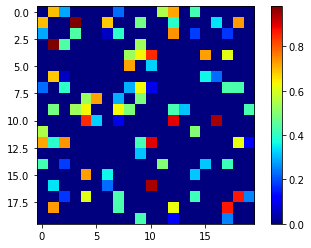
\includegraphics[width=\linewidth]{pictures/gt_A_heatmap.png}
  \end{subfigure}
  \begin{subfigure}[b]{0.4\linewidth}
    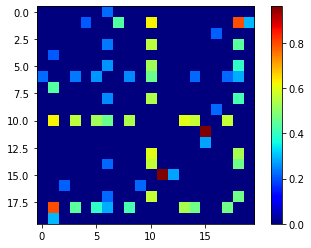
\includegraphics[width=\linewidth]{pictures/est_A_heatmap.png}
  \end{subfigure}
  \label{fig:heatmap}
\end{figure}

\begin{figure}
  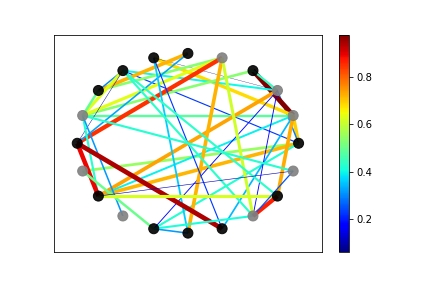
\includegraphics[width=\linewidth]{pictures/gt_graph.png}
  \caption{Graph estimated from synthetic data.}
  \label{fig:gt}
\end{figure}

\section{Discussion}

To our knowledge, this is the first work on learning graph topology from binary signals. We have developed a method to effectively learn the graph adjacency matrix from binary signals. This model can be easily extended for learning binomial signals in general. Incorporating parameter optimization techniques would be a natural improvement in this model. Moreover, it would be desirable to develop scalable algorithms that can be used to learn a topology for a large graph from signals. Recently, in \cite{saboksayr2021accelerated} the author shows fast proximal-gradient iterations can be applied to the framework given by \cite{kalofolias2016learn} improving the overall runtime.

\section*{Acknowledgment}

This work is supported by Research, Scholarship, and Creative Activity (RSCA) Award 2021-2022 through Chico State Enterprises. Thank you to Dr. Robin Donatello, Ph.D., for approving this work for Data Science Capstone Project.

\newpage

\bibliographystyle{IEEEtran}
\bibliography{ref}

\end{document}
